\documentclass[11pt,a4paper]{article}
\usepackage[margin=2.2cm]{geometry}
\usepackage[T1]{fontenc}
\usepackage{charter}
\usepackage{microtype}
\usepackage{graphicx}
\usepackage{booktabs}
\usepackage{array}
\usepackage{tabularx}
\usepackage{float}
\usepackage{caption}
\usepackage{enumitem}
\usepackage{amsmath}
\usepackage[table]{xcolor}
\usepackage{listings}
\usepackage[most]{tcolorbox}
\usepackage{fancyhdr}
\usepackage[colorlinks=true,linkcolor=accent,urlcolor=accent]{hyperref}

\definecolor{accent}{HTML}{3C3489}
\definecolor{codebg}{HTML}{F6F6F3}
\definecolor{kw}{HTML}{185FA5}
\definecolor{cm}{HTML}{6B6A64}
\definecolor{okgreen}{HTML}{0F6E56}
\definecolor{badred}{HTML}{A32D2D}

\setlength{\parindent}{0pt}
\setlength{\parskip}{6pt}
\setlist{itemsep=2pt,topsep=4pt}
\captionsetup{font=small,labelfont=bf}
\renewcommand{\arraystretch}{1.18}

\pagestyle{fancy}\fancyhf{}
\rhead{\small\color{cm}\reporttag}
\cfoot{\small\thepage}
\renewcommand{\headrulewidth}{0.3pt}

\lstdefinelanguage{SV}{
  morekeywords={module,endmodule,input,output,inout,logic,wire,reg,always_ff,always_comb,assign,
    begin,end,if,else,case,endcase,default,typedef,enum,localparam,posedge,negedge,or,task,endtask,
    function,endfunction,automatic,initial,repeat,while,for,integer,string,signed,void},
  sensitive=true, morecomment=[l]{//}, morecomment=[s]{/*}{*/}, morestring=[b]"}
\lstdefinelanguage{ICCTcl}{
  morekeywords={set_app_var,create_mw_lib,open_mw_lib,import_designs,read_sdc,set_tlu_plus_files,
    save_mw_cel,create_floorplan,derive_pg_connection,create_rectangular_ring,create_power_strap,
    create_fp_placement,place_opt,clock_opt,report_placement_utilization,report_qor,report_timing,
    insert_stdcell_filler,route_opt,verify_zrt_route,extract_rc,write_parasitics,write_verilog,
    close_mw_cel,gui_start,set_dont_use,get_lib_cells},
  sensitive=true, morecomment=[l]{\#}}
\lstset{basicstyle=\ttfamily\footnotesize, backgroundcolor=\color{codebg}, frame=single,
  rulecolor=\color{codebg}, keywordstyle=\color{kw}\bfseries, commentstyle=\color{cm}\itshape,
  columns=fullflexible, keepspaces=true, breaklines=true, showstringspaces=false,
  xleftmargin=4pt, xrightmargin=4pt, aboveskip=6pt, belowskip=6pt}

\newtcolorbox{task}{colback=accent!5,colframe=accent,boxrule=0.6pt,arc=2pt,
  left=8pt,right=8pt,top=4pt,bottom=4pt,fonttitle=\bfseries,title=The assignment}
\newtcolorbox{keypoint}[1]{colback=okgreen!6,colframe=okgreen,boxrule=0.6pt,arc=2pt,
  left=8pt,right=8pt,top=4pt,bottom=4pt,fonttitle=\bfseries,title={#1}}
\newtcolorbox{lesson}[1]{colback=orange!7,colframe=orange!70!black,boxrule=0.6pt,arc=2pt,
  left=8pt,right=8pt,top=4pt,bottom=4pt,fonttitle=\bfseries,title={#1}}

\newcommand{\fig}[3]{\begin{figure}[H]\centering\includegraphics[width=#2\linewidth]{figures/#1}\caption{#3}\end{figure}}
\newcommand{\met}{\textcolor{okgreen}{\textbf{MET}}}
\newcommand{\viol}{\textcolor{badred}{\textbf{VIOLATED}}}
% numbers still to be copied from my own .rpt files (shows in red until filled in)
\newcommand{\fillin}[1]{\textcolor{badred}{\textbf{[#1]}}}

\newcommand{\header}[3]{%
  \begin{center}
  {\small\color{cm} CPE 527 VLSI Design \quad|\quad Lab 3 \quad|\quad University of Alabama in Huntsville}\\[8pt]
  {\LARGE\bfseries\color{accent} #1}\\[4pt]
  {\large #2}\\[8pt]
  {\small Bibek Shrestha \quad|\quad October 2026 \quad|\quad #3}
  \end{center}\vspace{2pt}\hrule\vspace{6pt}}
\newcommand{\reporttag}{Lab 3 / Assignment 1: Fibonacci generator place and route}
\begin{document}
\header{Place and Route of the 16-bit Fibonacci Generator}{Taking the Lab 2 netlist through IC Compiler}{Synopsys IC Compiler, SAED 90\,nm}

\begin{task}
Run the IC Compiler flow from the tutorial on a design from the previous lab: floorplan, power plan,
placement, clock tree synthesis and routing. Generate and analyze the reports after CTS and after routing.
\end{task}

\section*{At a glance}
\begin{table}[H]\centering\small
\begin{tabular}{lccc}
\toprule
 & \textbf{Lab 2 (DC, area run)} & \textbf{After CTS} & \textbf{After routing} \\
\midrule
Library corner & typ & max & max \\
Wires & none & estimated & routed + extracted \\
Clock & 5 ns & 5 ns & 5 ns \\
Critical path & 4.35 ns & \fillin{ns} & \fillin{ns} \\
Setup slack & +0.56 ns & \fillin{ns} & \fillin{ns} \\
Violating paths & 0 & \fillin{} & \fillin{} \\
Hold violations & & \fillin{} & \fillin{} \\
Cells & 122 & \fillin{} & \fillin{} \\
Utilization & & \fillin{\%} & \fillin{\%} \\
Open nets / DRCs & & & \fillin{} / \fillin{} \\
\bottomrule
\end{tabular}
\caption{Lab 2 synthesis next to the two ICC checkpoints.}
\end{table}

\section{The design}
FIBO from Lab 2: three 16-bit registers (48 flip-flops) and one shared adder that produce 1, 1, 2, 3, 5, 8, \dots\
Ports: \texttt{clk}, \texttt{rst}, \texttt{en} and \texttt{OUT[15:0]}, 19 signal pins.

\fig{a1_block.png}{0.72}{Block diagram from Lab 2.}

\section{Script}
Same flow as the tutorial with new names (\texttt{FIBO\_LIB}, top \texttt{FIBO}, \texttt{fibo\_area.sdc}, checkpoints
\texttt{FIBO\_init}, \texttt{FIBO\_cts\_opt}, \texttt{FIBO\_route}). One real difference: the Lab 2 script for this
design never wrote a \texttt{.ddc}, so the Verilog netlist is imported instead.
\begin{lstlisting}[language=ICCTcl]
import_designs "../output/fibo_area_synth.v" -format verilog -top "FIBO" -cel "FIBO"
read_sdc ../constraints/fibo_area.sdc
\end{lstlisting}
A Verilog netlist has no constraints inside it, so \texttt{read\_sdc} is what brings in the 5\,ns clock.

\section{Routed layout}
\begin{figure}[H]\centering
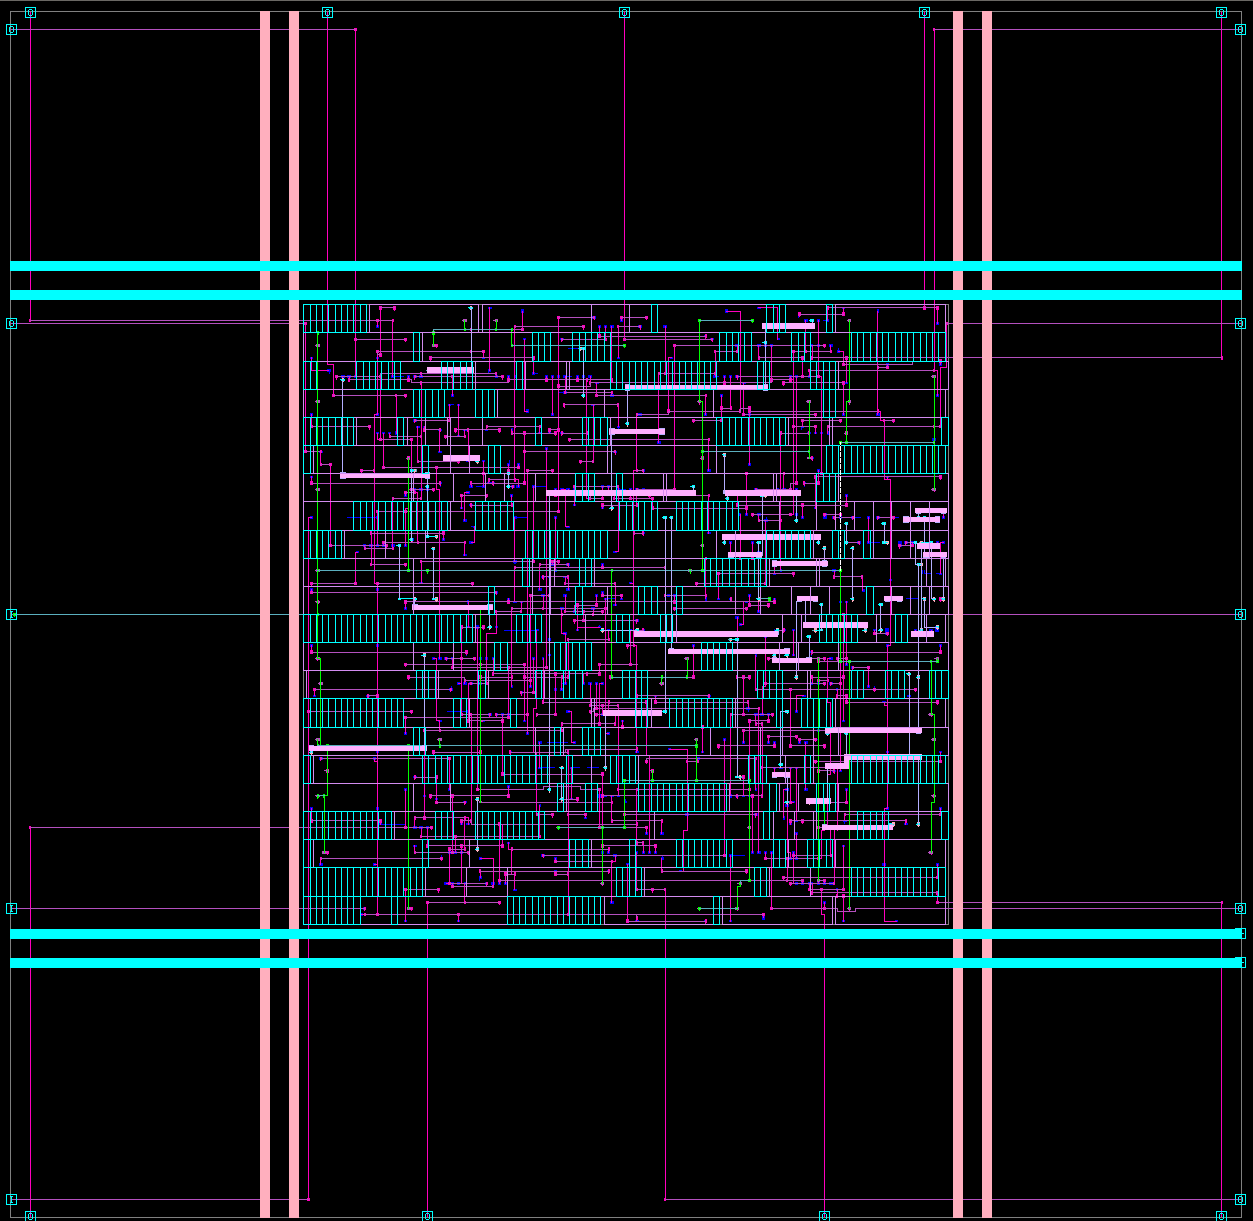
\includegraphics[width=0.45\linewidth]{figures/icc_routed.png}\hfill
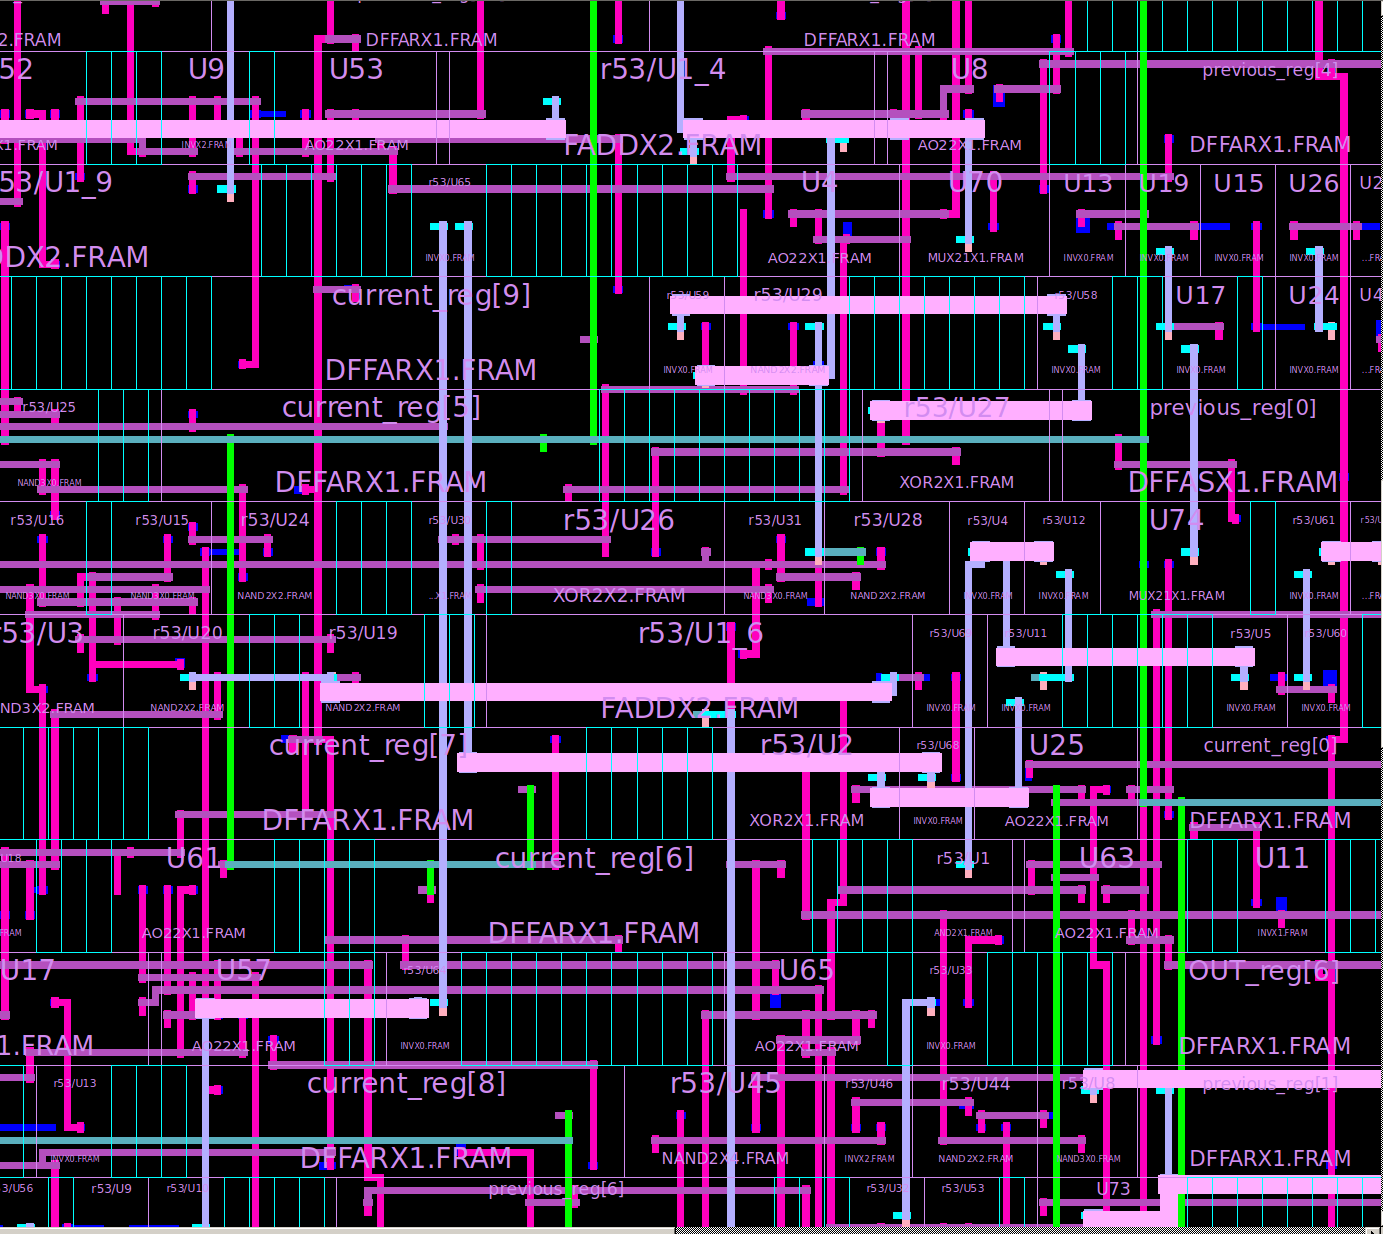
\includegraphics[width=0.53\linewidth]{figures/icc_routed_zoom.png}
\caption{Left: the routed block. Right: zoom on the core: adder stages \texttt{r53/U1\_4}, \texttt{r53/U1\_6}, \texttt{r53/U1\_9},
the \texttt{current\_reg} and \texttt{previous\_reg} flip-flops and \texttt{OUT\_reg[6]}.}
\end{figure}

\begin{itemize}
\item \textbf{Clock net.} Clicking a clock wire gives net \texttt{clk}, type Clock, layer M4, width 0.16\,\textmu m:
      after \texttt{clock\_opt} the clock is a real routed net, not an ideal signal any more.
\item \textbf{Reset value shows in the cells.} \texttt{previous} resets to 1, so \texttt{previous\_reg[0]} is a
      set-type \texttt{DFFASX1} while the other flip-flops are \texttt{DFFARX1}, the same mix Lab 2 reported.
\item \textbf{The adder keeps its name.} The full adders are still \texttt{r53/U1\_1} to \texttt{r53/U1\_15}, so the Lab 2
      critical path can be followed cell by cell in the layout.
\end{itemize}

\fig{fibo_path.png}{0.98}{The Lab 2 critical path. Every box is a cell that can be found by name in the routed layout.}

\section{Reports}
\begin{table}[H]\centering\small
\begin{tabular}{lll}
\toprule
Report & What I checked & Result \\
\midrule
\texttt{FIBO\_route\_qor.rpt} & slack, violating paths & \fillin{} \\
\texttt{FIBO\_route.setup.rpt} & worst setup path & \fillin{start $\rightarrow$ end, slack} \\
\texttt{FIBO\_route.hold.rpt} & worst hold path & \fillin{} \\
\texttt{FIBO\_route\_util.rpt} & standard cell utilization & \fillin{} \\
\texttt{verify\_zrt\_route} & open nets, DRCs & \fillin{} \\
\bottomrule
\end{tabular}
\caption{Post-route reports.}
\end{table}

\begin{lesson}{Compared with Lab 2}
The 0.56\,ns of slack in Lab 2 was at the typical corner with no wires. At the slow corner with routed wires
the same carry chain gives \fillin{ns} of slack, so the design \fillin{still meets / misses} 5\,ns.
\end{lesson}

\section{Inside the cells}
\fig{icc_faddx1_fram.png}{0.9}{\texttt{FADDX1}, FRAM view: the full adder repeated 14 times in the carry chain.
It has five pin squares (A, B, carry in, sum, carry out) and is one of the widest logic cells in the design.}

\section{What I learned}
\begin{itemize}
\item A Verilog netlist imports fine, but the constraints must come from the SDC.
\item Instance names from synthesis survive place and route, so a timing path from Design Compiler can be traced in the layout.
\item Reset values are visible in the hardware: one set-type flip-flop among 47 clear-type ones.
\end{itemize}

\appendix
\section{Source files}
\subsection*{RTL: \texttt{src/assignment2.sv}}
\lstinputlisting[language=SV]{src/assignment2.sv}
\subsection*{Testbench: \texttt{src/assignment2\_tb.sv}}
\lstinputlisting[language=SV]{src/assignment2_tb.sv}
\subsection*{ICC script: \texttt{src/icc\_fibo.tcl}}
\lstinputlisting[language=ICCTcl]{src/icc_fibo.tcl}
\end{document}
